\documentclass[a4paper, 11pt]{article}
% TeX-template
% Copyright (c) 2024 Joseph Tooby-Smith. All rights reserved.
% Released under Apache 2.0 license.
% Paper content: 
% Copyright (c) 2024 Joseph Tooby-Smith. All rights reserved.
\usepackage{xcolor}
\usepackage{setspace}

\onehalfspacing%
%\setstretch{3} % Custom separation of lines.
\renewcommand{\arraystretch}{1.5}
%%%%%%%%%%%%%%%%%%%%%%%%%%%%%%%%
%Hyperlinks
\usepackage{hyperref}
\definecolor{mycolor}{RGB}{0,88,204}
\hypersetup{
  colorlinks=true,
  linkcolor=mycolor,
  urlcolor=mycolor,
  citecolor=mycolor
}
%%%%%%%%%%%%%%%%%%%%%%%%%%%%%%%%
%Mathematics
\usepackage{amsmath}
%%%%%%%%%%%%%%%%%%%%%%%%%%%%%%%%
%Margins
\usepackage{geometry}

\geometry{
  top=0.8in,
  bottom=0.8in,
  left=1in,
  right=1in
}
%%%%%%%%%%%%%%%%%%%%%%%%%%%%%%%%
%Page numbers
\usepackage{fancyhdr}


\pagestyle{fancy}
\fancyhf{}
\fancyhead[R]{\thepage}
\renewcommand{\headrulewidth}{0pt}
\setlength{\headheight}{13.6pt}
%For the title page
\fancypagestyle{plain}{%
  \fancyhf{}
  \fancyhead[R]{\thepage}
  \renewcommand{\headrulewidth}{0pt}
}
%%%%%%%%%%%%%%%%%%%%%%%%%%%%%%%%
%Fonts

\usepackage{mathptmx}

%%%%%%%%%%%%%%%%%%%%%%%%%%%%%%%%
%Section style

\usepackage{titlesec}

\titleformat{\section}
  {\normalfont\large\centering}{\thesection.}{1em}{\MakeUppercase}
\titleformat{\subsection}
  {\normalfont\centering}{\thesubsection.}{1em}{\MakeUppercase}

  \titlespacing{\paragraph}{10pt}{0pt}{6pt}[0pt]
%%%%%%%%%%%%%%%%%%%%%%%%%%%%%%%%
%Comments

\newcommand{\js}[1]{ {\color{magenta} js:  #1}}

%%%%%%%%%%%%%%%%%%%%%%%%%%%%%%%%
%SVG images
\usepackage{svg}
%%%%%%%%%%%%%%%%%%%%%%%%%%%%%%%%
%Paragraph markers
%\newcommand{\paragraphMarker}[1]{ %{\color{gray} $\langle$#1$\rangle$}
%}
%%%%%%%%%%%%%%%%%%%%%%%%%%%%%%%
%Lean formating
\usepackage{listings}
\usepackage[T1]{fontenc}
\usepackage[utf8]{inputenc}
\usepackage{amssymb}
\usepackage{chngcntr}
\definecolor{keywordcolor}{rgb}{0.7, 0.1, 0.1}   % red
\definecolor{tacticcolor}{rgb}{0.0, 0.1, 0.6}    % blue
\definecolor{commentcolor}{rgb}{0.4, 0.4, 0.4}   % grey
\definecolor{symbolcolor}{rgb}{0.0, 0.1, 0.6}    % blue
\definecolor{sortcolor}{rgb}{0.1, 0.5, 0.1}      % green
\definecolor{attributecolor}{rgb}{0.7, 0.1, 0.1} % red

\def\lstlanguagefiles{lstlean.tex}
\lstset{
 	frame = lrtb,
 	rulecolor=\color{mycolor},
	language=lean,
	aboveskip = 5mm,
	belowskip = 5mm,
	captionpos=t
	}

\lstnewenvironment{code}[1][]%
{
   \noindent\newline
   \minipage{\linewidth}
   \vspace{0.5\baselineskip}
   \lstset{
 	frame = lrtb,
 	rulecolor=\color{mycolor},
 	escapeinside={/*!}{!*/},
	language=lean,
	aboveskip = 5mm,
	belowskip = 5mm,
	xleftmargin=2mm,
	xrightmargin=2mm,
	}
	}
{\endminipage\newline}
\lstnewenvironment{codeLong}[1][]%
{
   \lstset{
 	frame = lrtb,
 	rulecolor=\color{mycolor},
 	escapeinside={/*!}{!*/},
	language=lean,
	aboveskip = 5mm,
	belowskip = 5mm,
	xleftmargin=2mm,
	xrightmargin=2mm,
	}
	}
{}
%%%%%%%%%%%%%%%%%%%%%%%%%%%%%%%%
%Links in code block
% put at top of code block using
% /*!\codeLink{...}!*/
\newcommand{\codeLink}[1]{
  \vspace{-0.5cm}\hfill\href{https://github.com/HEPLean/HepLean/blob/1b951994ae3d882242b02d23957ef1ee7fa05f3d/HepLean/#1}{(source)}
  }
  \newcommand{\codeBreakdownLink}[2]{
  \vspace{-0.5cm}\hfill\href{https://github.com/HEPLean/HepLean/blob/1b951994ae3d882242b02d23957ef1ee7fa05f3d/HepLean/#1}{(source)}
  (breakdown \ref{#2})
  }
 \newcommand{\textLink}[1]{\href{https://github.com/HEPLean/HepLean/blob/1b951994ae3d882242b02d23957ef1ee7fa05f3d/HepLean/#1}{source}}
 \newcommand{\textLinkB}[1]{\href{https://github.com/HEPLean/HepLean/blob/1b951994ae3d882242b02d23957ef1ee7fa05f3d/HepLean/#1}{(source)}}
%%%%%%%%%%%%%%%%%%%%%%%%%%%%%%%%
%Title, author, date
\title{Index notation in Lean 4}
\author{Joseph Tooby-Smith \\ \textit{Affiliation}}
\date{\today}
%%%%%%%%%%%%%%%%%%%%%%%%%%%%%%%%

\begin{document}
\counterwithin{lstlisting}{section}
\maketitle
\vspace{-1cm}
\begin{abstract}
Index notation is tool commonly used in physics to manipulate tensors.
In physics, we use index notation for three different types of tensors: 
Einstein tensors (e.g., ordinary vectors and matrices), Lorentz tensors, and 
Van der Waerden tensors. In this paper, we discuss how these are implemented in Lean 4 using a 
general mathematical theory based on category theory, and related to the notation of an operad.
\end{abstract}


\section{Overview}
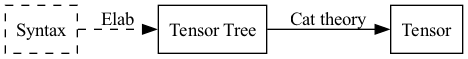
\includegraphics[width=\textwidth]{overviewFlow.png}

Index notation in Lean, and really in any language including pen and paper, involves three steps:
\section{Color}

One of the key features of our construction will be the notation of a color. 
A color is a property associated to an index.  
To start with an example, Lorentz tensors have two colors up and down, in other words an 
index can be an up-index or a down-index. Einstien tensors only have one index, and 
Van der Waerden tensors have six colors; two for left-handed fermions, two for right-handed 
fermions, and two for four-vector indices. 

We generically denote by $C$ the type of colors. As an example, for
Lorentz tensors $C = {up, down}$. 

Let $\mathcal{S}$ be the category of types (or sets). The category $\mathcal{S}_{/C}$ is the 
category 
of types over $C$, that is whose objects are maps $X\to C$ and whose morphisms from 
$X\to C$ to $Y\to C$ are maps $X\to Y$ making the obvious triangle diagram commutes. 

The core of $\mathcal{S}_{/C}$, denoted $\mathcal{S}_{/C}^\times$, can be thought of as the 
category of indexing sets of tensors of a given type. We will see this made manifest with 
a symmetric monoidal functor later.




\bibliographystyle{unsrturl}
\begin{spacing}{0.5}
\bibliography{MyBib}
\end{spacing}


%%%%%%%%%%%%%%
\end{document}
